\chapter{Vectors}
\label{vectors}

In the previous chapter we used a loop to compute the elements of a sequence, but we were only able to store the last element.  In this chapter, we'll use a vector to store all of the elements.
We'll also learn how to select elements from a vector, and how to perform vector arithmetic and common vector operations like reduce and apply.


\section{Creating Vectors}

\index{vector}

A \emph{vector} in MATLAB is a sequence of numbers.
There are several ways to create vectors; one of the most common is
to put a sequence of numbers in square brackets:

\begin{code}
>> ***[1 2 3]***
ans = 1     2     3
\end{code}

Another way to create a vector is the colon operator, which we have already used to create a range of values in a {\tt for} loop.

\begin{code}
>> ***1:3***
ans = 1     2     3
\end{code}

In general, anything you can do with a number, you can also do with
a vector.  For example, you can assign a vector value to a variable:

\begin{code}
>> ***X = [1 2 3]***
X = 1     2     3
\end{code}

Note that variables that contain vectors are often capital letters.
That's just a convention; MATLAB doesn't require it, but it's a useful way to remember which variables are vectors.

\index{variable}

\section{Vector Arithmetic}
\label{elementwise}

\index{vector arithmetic}
\index{arithmetic!vector}

As with numbers, you can do arithmetic with vectors.  If you add a number
to a vector, MATLAB increments each element of the vector:

\begin{code}
>> ***Y = X + 5***
Y = 6     7     8
\end{code}

\noindent The result is a new vector; the original value of {\tt X} has not
changed.

If you add two vectors, MATLAB adds the corresponding elements of each
vector and creates a new vector that contains the sums:

\begin{code}
>> ***Z = X+Y***
Z = 7     9    11
\end{code}

But adding vectors only works if the operands are the same size.
Otherwise you get an error:

\begin{code}
>> ***W = [1 2]***
W = 1     2     3

>> ***X + W***
Matrix dimensions must agree.
\end{code}

\noindent The error message in this case is confusing, because we think of these values as vectors, not matrices.
We'll come back to this topic later, but for now you can think of a vector as a kind of matrix.

\index{matrix}
\index{elementwise operator}
\index{operator!elementwise}

If you divide two vectors, you might be surprised by the result:

\begin{code}
>> ***X / Y***
ans = 0.4156
\end{code}

MATLAB is performing a matrix operation called right division; an explanation of right division is outside the scope of this book. If you want to divide the elements of {\tt X} by the elements of {\tt Y}, you have to use {\tt ./}, which is elementwise division:

\begin{code}
>> ***X ./ Y***
ans = 0.2500    0.4000    0.5000
\end{code}

Multiplication has the same problem.  If you use {\tt *}, MATLAB does matrix multiplication.  With these two vectors, matrix multiplication is not defined, and you get an error:

\begin{code}
>> ***X * Y***
Error using  * 
Incorrect dimensions for matrix multiplication. 
Check that the number of columns in the first matrix 
matches the number of rows in the second matrix
To perform elementwise multiplication, use '.*'.
\end{code}

In this case, the error message is pretty helpful.  As it suggests, you can use {\tt .*} to perform elementwise multiplication:

\index{matrix multiplication}
\index{multiplication!matrix}

\begin{code}
>> ***X .* Y***
ans = 4    10    18
\end{code}

As an exercise, see what happens if you use the exponentiation operator,
\verb"^", with a vector.

\section{Selecting Elements}

\index{element}
\index{parentheses}

You can select an element from a vector with parentheses:

\begin{code}
>> ***Y = [6 7 8 9]***
Y = 6    7     8     9

>> ***Y(1)***
ans = 6

>> ***Y(4)***
ans = 9
\end{code}

This means that the first element of {\tt Y} is 6 and the
fourth element is 9.
The number in parentheses is called the \emph{index} because it indicates which element of the vector you want.

\index{index}

The index can be a variable name or a mathematical expression:

\begin{code}
>> ***i = 1;***
>> ***Y(i)***
ans = 6
>> ***Y(i+1)***
ans = 7
\end{code}

We can use a loop to display the elements of {\tt Y}:

\index{loop}

\begin{code}
for i=1:4
     Y(i)
end
\end{code}

Each time through the loop we use a different value of {\tt i}
as an index into {\tt Y}.

\index{length function@{\tt length} function}
\index{function!{\tt length}}

In the previous example we have to know the number
of elements in {\tt Y}.  We can make it more general by using
the {\tt length} function, which returns the number of elements
in a vector:

\begin{code}
for i=1:length(Y)
     Y(i)
end
\end{code}

This version works for a vector of any length.


\subsection{Indexing Errors}

\index{index}
\index{expression}

An index can be any kind of expression, but the value of the
expression has to be a positive integer, and it has to be
less than or equal to the length of the vector.  If it's
zero or negative, you'll get an error:

\begin{code}
>> ***Y(0)***
Array indices must be positive integers or logical values.
\end{code}

If it's not an integer, you get an error:

\begin{code}
>> ***Y(1.5)***
Array indices must be positive integers or logical values.
\end{code}

If the index is too big, you also get an error:

\begin{code}
>> ***Y(5)***
Index exceeds the number of array elements (4).
\end{code}

The error messages use the word ``array'' rather than ``matrix'', 
but they mean the same thing, at least for now.

\index{array}

\section{Vectors and Sequences}
\label{vecseq}

\index{vector}
\index{sequence}
\index{Fibonacci}

Vectors and sequences go together nicely.
For example, another way to evaluate the Fibonacci sequence from Chapter 2 is to
store successive values in a vector.  Remember that the definition of the
Fibonacci sequence is $F_1 = 1$, $F_2 = 1$, and
$F_{i} = F_{i-1} + F_{i-2}$ for $i > 2$.

Listing~\ref{lst:fib_vec} shows how we can compute the elements of this sequence and store them in a vector.

\begin{lstlisting}[caption={Calculating the Fibonacci sequence using a vector }, label={lst:fib_vec}]
F(1) = 1
F(2) = 1
for i=3:n
    F(i) = F(i-1) + F(i-2)
end
\end{lstlisting}

I use a capital letter for the vector {\tt F}
and lower-case letters for the integers {\tt i} and {\tt n}.

If you had any trouble with Exercise~\ref{fib2}, you have to
appreciate the simplicity of this script.  The MATLAB syntax is
similar to the math notation, which makes it easier to check
correctness.  

If you only want the $n$th Fibonacci number, storing
the whole sequence wastes some space.  But if wasting space
makes your code easier to write and debug, that's probably ok.


\section{Plotting Vectors}

\index{plotting vector}
\index{vector!plotting}
\index{plot@{\tt plot}}

If you call {\tt plot} with a vector as an argument,
MATLAB plots the indices on the $x$-axis and the elements on the
$y$-axis.  To plot the Fibonacci numbers we computed in Listing~\ref{lst:fib_vec}, we'd use:

\begin{code}
plot(F)
\end{code}

Figure~\ref{fig:fibonacci} shows the result.

\begin{figure}[h]
\centerline{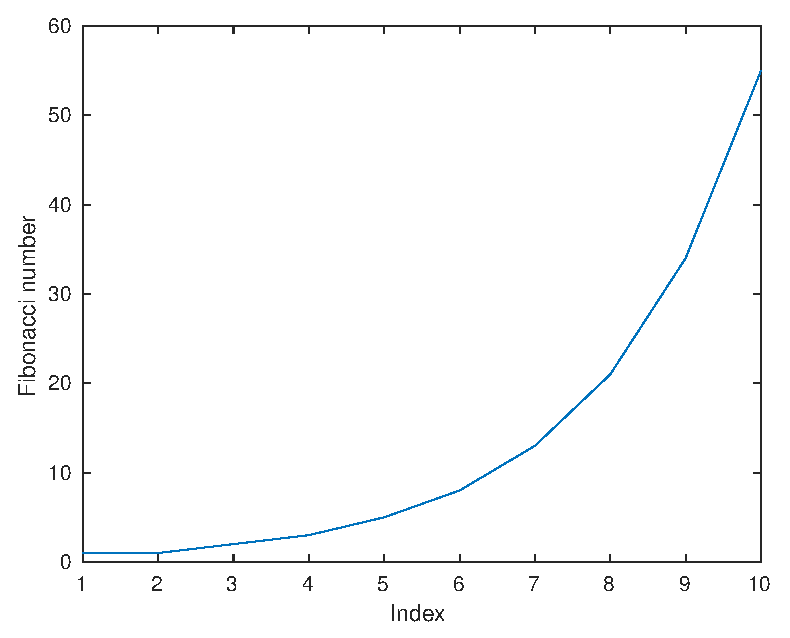
\includegraphics[height=3in]{book/figs/fibonacci.eps}}
\caption{The first 10 elements of the Fibonacci sequence.}
\label{fig:fibonacci}
\end{figure}

This way of looking at a vector is often useful for debugging, especially
if it is big enough that displaying the elements on
the screen is unwieldy.


\section{Common Vector Operations}

We've covered some of the basic features of vectors. Let's now look at some common patterns we use to work with data stored in vectors.

\subsection{Reduce}
\label{reduce}

We frequently use loops to run through the elements of a vector
and add them up, multiply them together, compute the sum
of their squares, and so on.  This kind of operation is called \emph{reduce},
because it reduces a vector with multiple elements down to a single
number.

\index{reduce}
\index{vector}

For example, the loop in Listing~\ref{lst:vec_reduce} adds up the elements of a vector named {\tt X} (which we assume has been defined).

\begin{lstlisting}[caption={Reducing a vector to a single scalar value (the sum)}, label={lst:vec_reduce}]
total = 0
for i=1:length(X)
    total = total + X(i)
end
ans = total
\end{lstlisting}

The use of {\tt total} as an accumulator is similar to what we
saw in Chapter 3.  Again, we use the {\tt length} function
to find the upper bound of the range, so this loop will work
regardless of the length of {\tt X}.
Each time through the loop, we add
in the {\tt i}th element of {\tt X}, so at the end of the loop
{\tt total} contains the sum of the elements.

\index{accumulator}
\index{length function@{\tt length} function}

MATLAB provides functions that perform some reduce operations.
For example, the {\tt sum} function computes the sum of the elements
in a vector and {\tt prod} computes the product.


\subsection{Apply}
\label{apply}

Another common use of a loop is to run through the elements of
a vector, perform some operation on the elements, and create
a new vector with the results.  This operation is called
\emph{apply}, because you apply the operation to each element in
the vector.

\index{apply}

For example, the loop in Listing ~\ref{lst:vec_apply} creates a vector {\tt Y} that
contains the squares of the elements of {\tt X} (assuming, again, that {\tt X} is already defined).

\begin{lstlisting}[caption={Making a new vector Y by squaring the elements in X }, label={lst:vec_apply}]
for i=1:length(X)
    Y(i) = X(i)^2
end
\end{lstlisting}

Many apply operations can be done with elementwise operators.
The following statement is more concise than the loop in
Listing~\ref{lst:vec_apply}.

\begin{code}
Y = X .^ 2
\end{code}

It also runs faster!


\section{Summary}

In this chapter we used a vector to store the elements of a sequence.  We learned how to select elements from a vector and perform vector arithmetic.  We performed reduce and apply operations using {\tt for} loops, MATLAB function, and elementwise operations.

In the next chapter, you'll learn the most important idea in computer programming: functions!

Here are some terms from this chapter you might want to remember.

A compound statement is a statement, like {\tt if} and {\tt for}, that
contains other statements in an indented body.
If you put one compound statement in the body of another, they are ``nested''.

A scalar is single value; a vector is a sequence of values, and a matrix is a two-dimensional collection of values (also called ``array'' in some MATLAB documentation).

An index is an integer value used to indicate one of the elements
in a vector or matrix (also called ``subscript'' in some MATLAB documentation).

An operation is ``elementwise'' if it acts on the individual elements of a vector or matrix (unlike some linear algebra operations).

You can ``search'' a vector for an element that has some desired property.
You can ``apply'' an operation to all elements of a vector, and you can ``reduce'' a vector
to a single value, for example by computing the sum of the elements.

A name collision is a scenario where two scripts that use the same variable name interfere with each other.


\section{Exercises}

\begin{ex}
Write a loop that computes the first {\tt n} elements
of the geometric sequence $A_{i+1} = A_i/2$ with $A_1 = 1$.  Notice that
math notation puts $A_{i+1}$ on the left side of the equality.
When you translate to MATLAB, you might want to rewrite it with
$A_{i}$ on the left side.
\end{ex}

\begin{ex}
Write an expression that computes the square root of the sum of the squares of the elements of a vector, without using a loop.

\index{square root}
\end{ex}

\begin{ex}
\label{fibratio}

The ratio of consecutive Fibonacci numbers, $F_{n+1}/F_{n}$, converges
to a constant value as $n$ increases.  Write a script that computes
a vector with the first $n$ elements of a Fibonacci sequence (assuming
that the variable {\tt n} is defined), and then computes a new
vector that contains the ratios of consecutive Fibonacci numbers.
Plot this vector to see if it seems to converge.  What value does
it converge on?

\index{Fibonacci}

% fibonacci4.m
\end{ex}

\begin{ex}
  The following set of equations is based on a famous example of a chaotic system, the Lorenz attractor (see \url{https://greenteapress.com/matlab/lorenz}):
%
\begin{eqnarray}
x_{i+1} &=& x_i + \sigma \left( y_i - x_i \right) dt  \\
y_{i+1} &=& y_i + \left[ x_i (r - z_i) - y_i \right] dt   \\
z_{i+1} &=& z_i + \left( x_i y_i - b z_i \right) dt
\end{eqnarray}
%
\begin{itemize}

\item Write a script that computes the first 10 elements of the sequences
$X$, $Y$, and $Z$ and stores them in vectors named {\tt X}, {\tt Y},
and {\tt Z}.

Use the initial values $X_1 = 1$, $Y_1 = 2$, and $Z_1 = 3$, with values
$\sigma = 10$, $b = 8/3$, and $r = 28$, and with $dt = 0.01$.

\item Read the documentation for {\tt plot3} and {\tt comet3} and
plot the results in 3 dimensions.

\item Once the code is working, use semi-colons to suppress the output
and then run the program with sequence length 100, 1000, and 10000.

\item Run the program again with different starting conditions.
What effect does it have on the result?

\item Run the program with different values for $\sigma$, $b$, and $r$
and see if you can get a sense of how each variable affects the
system.

\end{itemize}

\index{Lorenz attractor}
% lorenz.m
\end{ex}


\begin{ex}
The logistic map (see \url{https://greenteapress.com/matlab/logistic}) is described by the following equation:

\index{logistic map}

\begin{equation}
X_{i+1} = r X_i (1-X_i)
\end{equation}

where $X_i$ is a number between zero and one and $r$ is a positive number.

\begin{itemize}

\item Write a script named {\tt logmap} that computes the first 50
elements of $X$ with {\tt r=3.9} and {\tt X1=0.5}, where
{\tt r} is the parameter of the logistic map and {\tt X1} is the
initial value.

\item Plot the results for a range of values of $r$ from 2.4 to 4.0.
How does the behavior of the system change as you vary $r$?

\end{itemize}

% logmap.m
\end{ex}


